\chapter{Problem statement} \label{chap:problem-statement}

In this chapter we firstly state the $PSm \;|\; intree \;|\; \sum_{j} w_j T_j$ variant of the \ac{rcpsp}.
Following this, we describe a constraint-programming method used to find solutions to the problem.
Lastly, we present a formal framework for identifying bottlenecks, relaxing related constraints,
and obtaining improved solutions.

% ~~~~~~~~~~~~~~~~~~~~~~~~~~~~~~~~~~~~~~~~~~~~~~~~~~~~~~~~~~~~~~~~~~~~~~~~~~~~~~~~~~~~~~~~~~~~~~~~~~~~~~~~~~~
\section{Scheduling} \label{sec:scheduling}

We use the $PSm \;|\; intree \;|\; \sum_{j} w_j T_j$ problem\footnote{Schema defined by \citet{BRUCKER1999}.}
to model the targeted real-world scheduling problem.
Additionally, we extend the problem by introducing several new definitions to better model the addressed problem.
Furthermore, we  introduce the notion of problem instances to help us distinguish between the original problem
and its modifications, as described in \cref{sec:alternative-schedule}.

A \emph{Problem instance} is a 4-tuple $\Instance = (\Jobs, \Precedences, \Resources, \horizon)$,
where

\begin{itemize}
    \item $\Jobs = \{1, \dots, n\}$ is a set of \emph{jobs},
    \item $\Precedences$ is a set of all \emph{precedences} constraints,
    \item $\Resources = \{1, \dots, m\}$ is a set of \emph{resources},
    \item $\horizon$ is the time horizon of the problem.
\end{itemize}

Each job $j \in \Jobs$ has an execution \emph{duration} $\duration{j}$,
describing the amount of time needed to process the job $j$.
\emph{Preemption} of jobs is not allowed
--- the execution of an job cannot be interrupted after its start.
Each job $j$ also has a \emph{deadline} $\deadline{j}$,
stating a time horizon in which the job should be completed;
otherwise, it is considered \emph{tardy}.
Subsequently, each job $j$ also has a \emph{tardiness weight} $\tardinessweight{j}$
which defines a penalty accumulated for each unit of time the job is tardy for.

Execution order of jobs is constrained with \emph{precedence constraints} $\Precedences$.
A precedence constraint between jobs $i$ and $j$, denoted as $\precedence{i}{j}$ or $(i, j)$,
states that processing of job $j$ can start only after the processing of job $i$ was completed.

Interpreting jobs $\Jobs$ as vertices and precedences $\Precedences$ as edges between the jobs,
we define the \emph{precedence graph} $G = (\Jobs, \Precedences)$.
We assume the precedence graph to be an \emph{inforest}, in other words,
the precedences constrain the execution order of jobs in such a way that the resulting precedence graph
is always an inforest.
An inforest is a directed acyclic graph where each vertex has at most one successor.
A connected subgraph of an inforest is an \emph{intree}.

Jobs are executed on \emph{resources} $\Resources$ --- machines with time-variant renewable \emph{capacities}.
Capacity of a resource $k$ during a time period $t$ is denoted as $\capacity{k}{t}$.
During their execution, jobs consume the capacities of resources.
For a job $j$, the per-period consumption of a resource $k$ is denoted as $\consumption{j}{k}$.
This describes how much of the resource's capacity is consumed each period during the job's execution.
Capacities are renewable, meaning that each time period the specified amount of capacity is available,
regardless of prior capacity consumptions.
The resource capacity functions $\capacity{k}{t}$ are assumed periodical with the same period
and the only value they take are $0$ and $\shiftcapacity{k} \negmedspace>\! 0$ for each corresponding resource $k$.
This assumption, however, is only for the initial problem instance
--- resource capacity functions of modified instances, as described in \cref{sec:alternative-schedule},
can be non-periodical and take arbitrary integer values.

The set of orders $\Orders = \{ j \in \Jobs \mid \nexists i : \precedence{j}{i} \}$
is the set of roots of the precedence intrees,
i.e. the set of all jobs for which no precedence successor exists.
If a job is contained in the set of orders $\Orders$, we call it an \emph{order}.

We make a simple observation; due to the intree-structure,
each (weakly) connected component in the precedence graph contains exactly one order.
From this, we can say that each job is associated with a specific order,
where associated states that the job is in the same component as that order.

Having introduced orders, we can now specify the ranges of job deadlines and tardiness weights
based on whether a job belongs to the orders set $\Orders$:

$$
\deadline{j} \begin{cases}
    \in \N    &\dots\;   j     \in \Orders \\
    +\infty   &\dots\;   j \not\in \Orders
\end{cases}
\qquad
\tardinessweight{j} \begin{cases}
    \geq 0   &\dots\;   j     \in \Orders \\
       = 0   &\dots\;   j \not\in \Orders
\end{cases}
$$

% ~~~~~~~~~~~~~~~~~~~~~~~~~~~~~~~~~~~~~~~~~~~~~~~~~~~~~~~~~~~~~~~~~~~~~~~~~~~~~~~~~~~~~~~~~~~~~~~~~~~~~~~~~~~
\section{Constraint programming model} \label{sec:constraint-programming-model}

We formulate the problem using a constraint programming model.
This provides us with a well-functioning framework
and allows us to use existing solvers for finding optimal solutions.

\begin{align}
    \text{given}      && \multicolumn{4}{l}{$\Jobs = (1, \dots, n) ,\;%
                                             \Resources = (1, \dots, m) ,\;%
                                             \Precedences ,\;%
                                             $} \nonumber \\
                      && \multicolumn{4}{l}{$\duration{1}, \dots, \duration{n} \in \Nzero ,\;%
                                             \deadline{1}, \dots, \deadline{n} \in \intinterval{0}{\horizon} ,\;%
                                             \tardinessweight{1}, \dots, \tardinessweight{n} \in \Nzero ,\;%
                                             $} \nonumber \\
                      && \multicolumn{4}{l}{$\consumption{1}{1}, \dots, \consumption{n}{m} \in \Nzero ,\;%
                                             \capacityf{1}, \dots, \capacityf{m} : \intinterval{0}{\horizon} \to \Nzero %
                                             $} \nonumber \\
    \text{find}       && \multicolumn{4}{l}{$\Schedule = (\jobstart{1}, \dots, \jobstart{n}) \in \N^n$} \nonumber \\
    \text{minimizing} && \sum_{j \in \Jobs} \tardinessweight{j} \tardiness{j}
                      &
                      &&
                      \label{csp:objective} \\
    \text{subject to} && \jobend{i}
                      & \leq \jobstart{j}
                      && \forall \precedence{i}{j} \in \Precedences
                      \label{csp:precedences} \\
                      && \sum_{j \in \Jobs} \modelConsumption{j}{k}{t}
                      & \leq \capacity{k}{t}
                      && \forall t \in 1, \dots, \horizon \; \forall k \in \Resources
                      \label{csp:capacities} \\
    \text{where}      && \multicolumn{4}{l}{$\Completions = (\jobstart{1} + \duration{1}, \dots, \jobstart{n} + \duration{n}) ,\;%
                                             \tardiness{j} = \max(0, \jobend{j} - \deadline{j}) ,\;%
                                             $} \nonumber \\
                      && \multicolumn{4}{l}{$\modelConsumption{j}{k}{t} \defeq \begin{cases}
                                                 \consumption{j}{k} & \jobstart{j} \leq t < \jobend{j} \\
                                                 0                  & \text{otherwise}
                                                 \end{cases}
                                             $} \nonumber
\end{align}

Inequalities \eqref{csp:precedences} formulate the precedence constraints --- start and end times of jobs
are according to all the precedences.
Inequalities \eqref{csp:capacities} formulate the resource capacity constraints --- in every time period
the combined consumption of jobs scheduled during the period cannot exceed any of the resource's capacities.
Expression \eqref{csp:objective} is the optimization minimization objective --- the weighted tardiness of jobs.

We assume we have a black-box solver available,
which is able to find solutions to the problem modeled through constraint-programming in reasonable time.

In the following sections, we will consider the stated constraints as potential bottlenecks
and how to relax specific constraints should they be identified as bottlenecks.

% ~~~~~~~~~~~~~~~~~~~~~~~~~~~~~~~~~~~~~~~~~~~~~~~~~~~~~~~~~~~~~~~~~~~~~~~~~~~~~~~~~~~~~~~~~~~~~~~~~~~~~~~~~~~
\section{Bottlenecks} \label{sec:bottlenecks}

Our goal will be to find bottlenecks in the problem, specifically in the obtained schedule
--- in the solution to the constraint-programming model defined in \cref{sec:constraint-programming-model}.
Firstly, we state a general definition of a execution-level bottleneck:

\begin{defn*}[\acf{ebm} \citep{WANG2016}]\label{def:bottleneck}
    \emph{\ac{ebm}} is a machine that dominates the scheduling performance in the strongest manner
    at the execution level of production systems.
\end{defn*}

The execution level of a production system stated here refers to finding bottlenecks
specific to the given problem instance and the obtained solution to that instance.
This is consistent with our goal of finding bottlenecks in the specific problem instances and their solutions,
and improving the performance of the system only with respect to the currently presented problems.
In contrast, we will not be interested in bottlenecks of the whole system
nor in generally improving the performance of the system regardless of the problem.
Having made the distinction, we will now discuss our interpretation of the definition suited to our problem.

Instead of identifying just a single machine as a bottleneck
or listing all the machines in the order of their scheduling impact,
we will focus on identifying specific time periods on specific machines as schedule bottlenecks.
This allows us to relax only the specific constraints related to the identified time periods,
resulting in localized modifications with minimal costs.

With focusing on constraints related to resources during specific time periods,
we are limited to considering only the resource capacity constraints \eqref{csp:capacities}.
Those constraints limit the cumulative consumption of jobs scheduled during a given time period
to be no more than the available capacities of all the resources during that time period,
constrained for each of the resources separately.

The cumulative consumption is dependent on the constructed schedule and the given problem instance.
Its value changes significantly with changing of the schedule,
which is an essential part of the black-box scheduling process.
This process is guided by the objective expression \eqref{csp:objective} and cannot be influenced.
Although the job tardiness weights $\tardinessweight{j}$ can potentially be changed,
we consider those as part of the problem definition,
stating the predefined importance of each of the orders,
and thus we will not allow their modifications.
Equally, job resource consumptions $\consumption{j}{k}$ influence the cumulative value,
but due to the nature of our problem,
we cannot modify the resource consumptions as those are predefined by the corresponding real-life
execution and operation requirements.

On the contrary, available capacities of resources can be modified with reasonable correspondence
to modifications of the real-life problem.
More specifically, capacity of a resource during a time period can be increased or decreased.
Increasing the capacity of a resource during specific time periods could correspond to increasing
the number of workers operating the resource machine,
assuming that increasing the number of operating workers increases the total processing capacity.
While sole reduction of capacities would not relax the constraints much, rather tighten them,
decreasing capacity of one resource by a specific amount while increasing the capacity of another resource
by the same amount could tighten the constraints on the former resource but relax the constraints on the later.
This decreasing of the capacity of one resource while increasing the capacity of another by the same amount
could correspond to migrating workers between the resource machines,
assuming that the changes of operating workers are possible.

We will consider \emph{capacity additions} and \emph{capacity migrations} as the possible relaxations
of scheduling constraints, namely of the constraints \eqref{csp:capacities}.
Additions are executed by increasing the capacity of a selected resource
by a specified amount over a specified time interval.
Migrations are executed by decreasing the capacity of a selected source resource
by a specified amount over a specified time interval
and increasing the capacity of a selected target resource
by the specified amount over the same time interval.
Illustrative example of a capacity addition and a capacity migrations is shown in \cref{fig:CapacityChanges}.

\begin{figure}
    \centering
    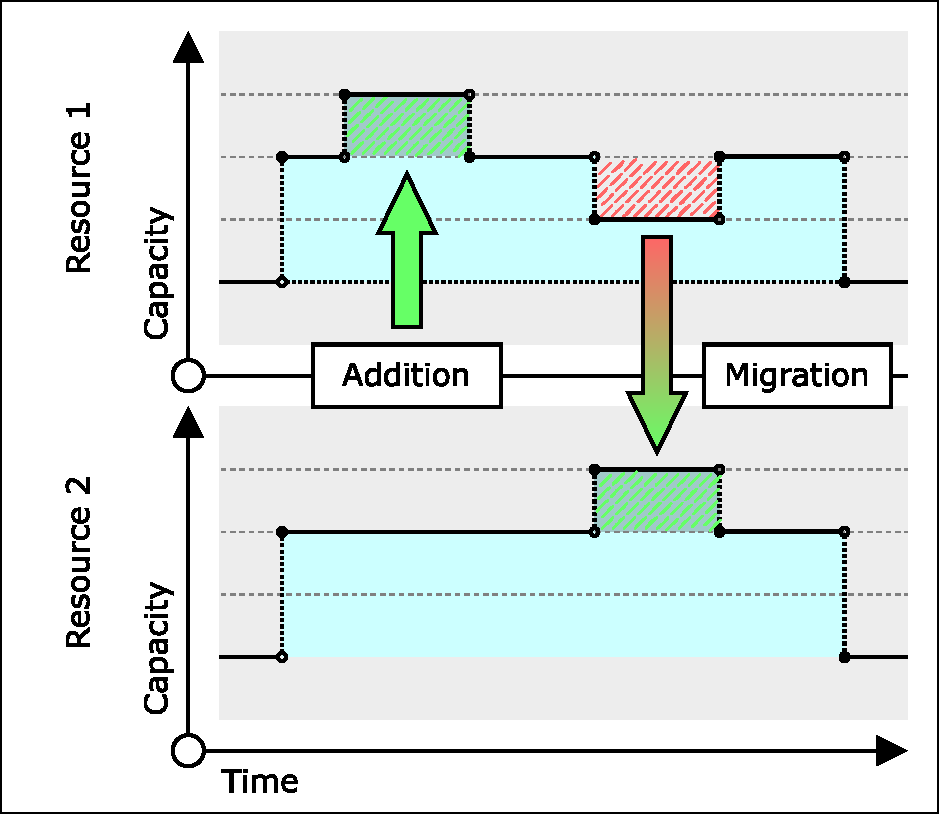
\includegraphics[width=0.7\textwidth]{img/Capacities-Changes.pdf}
    \caption{Diagram of possible capacity changes}
    \label{fig:CapacityChanges}
\end{figure}

We denote a capacity addition as $\addition{k}{s}{e}{c}$, where
$k$ is the resource whose capacity is increased,
$s$ and $e$ form the time interval $\intinterval{s}{e}$ over which the addition is executed, and
$c$ is the added capacity.
Analogously, we denote a capacity migration as $\migration{k_{\text{from}}}{k_{\text{to}}}{s}{e}{c}$, where
$k_{\text{from}}$ is the source resource whose capacity is lowered,
$k_{\text{to}}$ is the target resource whose capacity is increased,
$s$ and $e$ form the time interval $\intinterval{s}{e}$ over which the migration is executed, and
$c$ is the migrated capacity.
For a modified instance $\Instance^*$, the sets of all migrations and additions are denoted as
$\Migrations^{\Instance^*}$ and $\Additions^{\Instance^*}$, respectively.

% ~~~~~~~~~~~~~~~~~~~~~~~~~~~~~~~~~~~~~~~~~~~~~~~~~~~~~~~~~~~~~~~~~~~~~~~~~~~~~~~~~~~~~~~~~~~~~~~~~~~~~~~~~~~
\section{Alternative schedule} \label{sec:alternative-schedule}

In the rest of this chapter, we define a general procedure for solving the presented problem,
identifying bottlenecks and relaxing corresponding constraints by modifying the initial problem,
solving the modified problem,
and evaluating whether the modified solution reached a desired improvement.
More precisely:

\begin{enumerate}
    \item Suppose we obtained an optimal solution $\Schedule$ to the problem instance $\Instance$.

    \item We select a target order $\targetOrder \in \Orders$ for which to improve tardiness.
        We consider improvement to be any non-zero decrease in the objective function with respect to the
        selected order $\targetOrder$ and its tardiness $\tardiness{\targetOrder}$.

    \item We identify bottlenecks in the solution $\Schedule$ of the instance $\Instance$.

    \item Based on the identified bottlenecks, corresponding constraints are relaxed via
        capacity additions and capacity migrations.
        Those capacity changes are captured by modified resource capacity functions
        $\capacityf{1}^*, \ldots, \capacityf{m}^*$.
        With these modified capacity functions a modified problem instance $\Instance^*$ is constructed.

    \item We obtain a solution $\Schedule^*$ to the modified problem instance $\Instance^*$.

    \item Finally, any desired evaluations can be made on the modified solution $\Schedule^*$,
        alongside comparisons to the original solution $\Schedule$.
\end{enumerate}
